\subsubsection{Domain-klasse: Log}

Loggen har til formål at kunne lokalisere og identificere fejl i systemet. Loggen skal oprettes mere eller mindre globalt og der skal efterfølgende medgives en pointer til samtlige klasser på Pi. Alle disse klasser skal således anvende loggen som debugging redskab. Der skal som udgangspunkt kun skrives i loggen hvis en fejl opstår, da loggen ellers bliver uoverskuelig. Når der skrives til loggen, anvender den pågældende tråd cpu-tid, hvilket ligeledes er en grund til at være opmærksom på hvornår det er smart at skrive til loggen. \\
For at forhindre at log-entries fra forskellige tråde sammenflettes, skal der i implementeringen anvendes \texttt{std::mutex} som lås når der skrives i loggen.

\begin{figure}[h]
\centering
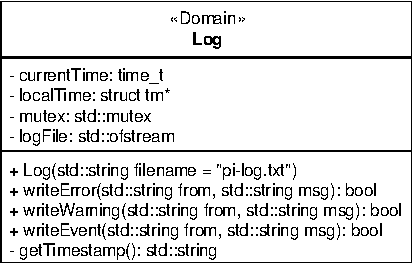
\includegraphics[]{../fig/diagrammer/bil/cd_log.pdf}
\caption{Klassebeskrivelse for domain-klassen Log}
\label{fig:cd_log}
\end{figure}

\textbf{Attributter}

\begin{table}[h]
\begin{tabularx}{\textwidth}{| Z | Z | L{10cm} |} \hline
Navn & Type & Beskrivelse \\\hline

\texttt{currentTime} & \texttt{time\_t} &Denne attribut bruges til at gemme det nuværende tidspunkt, når \texttt{getTimestamp} kaldes. \\\hline

\texttt{localTime} & \texttt{struct tm*} & Anvendes til at holde tiden i et læseligt format. \\\hline

\texttt{mutex} & \texttt{std::mutex} & Anvendes som lås i \texttt{std::lock\_guard} der forhindrer flere tråde i at skrive i loggen på samme tid. \\\hline

\texttt{logFile} & \texttt{std::ofstream} & File descriptor til logfilen. \\\hline

\end{tabularx}
\caption{Attributter for klassen Log}
\label{table:attr_log}
\end{table}


\textbf{Metoder}
%------------------------------------- Log -------------------------------------
\begin{table}[h]
\begin{tabularx}{\textwidth}{| L{2.5 cm} | Z |} \hline
Prototype & \texttt{bool klassenavn(int velocity)} \\\hline
Parametre & \texttt{velocity} \newline Den hastighed der skal indlæses. \\\hline
Returværdi &  \texttt{bool} \newline Returnerer \texttt{true} hvis skrivningen er gået godt og \texttt{false} hvis skrivningen gik galt. \\\hline
Beskrivelse & Metoden indlæser den nyeste værdi af hastigheden i datastrukturen. \\\hline
\end{tabularx}
\caption{Metodebeskrivelse for \texttt{klassenavn}}
\label{table:met_klassenavn}
\end{table}

